\documentclass{article}
\usepackage{tikz}
\usetikzlibrary{arrows.meta,positioning,calc,shapes.geometric}
\pagestyle{empty}
\begin{document}
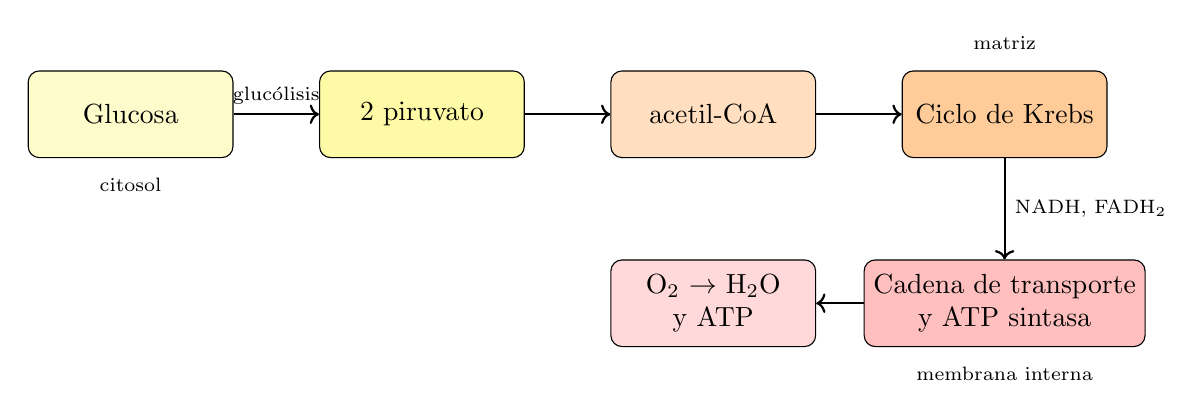
\begin{tikzpicture}
\tikzset{every node/.append style={align=center}}

\def\bx#1#2#3#4{\node[draw, rounded corners, fill=#4, minimum width=2.6cm, minimum height=1.1cm, align=center] (#1) at (#2) {#3};}
\bx{g}{0,0}{Glucosa}{yellow!20}
\bx{p}{3.7,0}{2 piruvato}{yellow!35}
\bx{a}{7.4,0}{acetil-CoA}{orange!25}
\bx{k}{11.1,0}{Ciclo de Krebs}{orange!40}
\bx{e}{11.1,-2.4}{Cadena de transporte\\ y ATP sintasa}{red!25}
\bx{o}{7.4,-2.4}{O$_2$ $\to$ H$_2$O\\ y ATP}{red!15}
\draw[->, thick] (g) -- node[above, font=\scriptsize] {glucólisis} (p);
\draw[->, thick] (p) -- (a); \draw[->, thick] (a) -- (k);
\draw[->, thick] (k) -- node[right, font=\scriptsize] {NADH, FADH$_2$} (e);
\draw[->, thick] (e) -- (o);
\node[font=\scriptsize] at (0,-0.9) {citosol}; \node[font=\scriptsize] at (11.1,0.9) {matriz}; \node[font=\scriptsize] at (11.1,-3.3) {membrana interna};

\end{tikzpicture}
\end{document}
